\chapter{Experiments}
\label{chap:experiments}

In this chapter we put both analysed methods (RP and $\Delta$RP) at work by detecting outliers in multivariate time series considerably more realistic than synthetically generated from sinusoidal functions. In section \ref{sec:experiments_setup} we discuss the data, performance metrics and parameter settings we used to do so. The results are presented in section \ref{sec:experiments_results}. We also examine the applicability of the RP-based methods on non-temporal data streams by using (non-temporal) data sets commonly used for benchmarking unsupervised (offline) outlier detection methods. The results of these experiments are presented and discussed in section \ref{sec:experiments_beyond}. We conclude this chapter with the key findings and final remarks.

\section{Experimental setup}
\label{sec:experiments_setup}

In chapter \ref{chap:analysis} we already got a good impression of the effectiveness of the methods with regard to the challenges imposed by the task of unsupervised online outlier detection in multivariate time series. Yet two evaluation criteria derived from these challenges were left open by the analysis. First, we want to assess the methods on realistic data and evaluate to what extent their performances depend on the structure of the data. Second, we want to determine the influence of $d$ and $n$ on the detection performance. In this chapter we focus mostly on those two criteria.

\subsection{Data}
To assess the performance of RP, $\Delta$RP and the considered baseline SPIRIT in a real-world context, we used a data set that consists of multiple time series generated by $24$ sensors measuring one water treatment plant (at the same time) \cite{goh2016dataset}. Other data sets commonly used for benchmarking outlier detection in time series such as the Yahoo Web Scope data set \cite{yahoo2015s5} and an outlier-version of the IntelLab data set \cite{bruijn2016benchmark} were not suitable due to the uncorrelated nature of the time series or a limited number of time series, respectively.

The water treatment plant data is originally created for research to cyber attack prevention. Unfortunately, the provided labellings were not aligned with the actual outliers due to a delay between the attack and the actual disruption of the system. Luckily, an attack-free version can be found online as well enabling us to inject the general types of outliers we focused on throughout this thesis ourselves. 

The data set consists of $n=496.800$ data points and $d=24$ time series from sensor readings that measured different parts of the water treatment plant\footnote{The data set also provides actuator readings which were excluded from the data.}. We used the readings of $4$ sensors that measured the same system component, and therefore are sufficiently correlated. We extracted only a fraction of $20.000$ data points from this data set and downsampled the result to a data set of $2.000$ data points.  

The $4$ time series do not have $0$ mean and the ranges of the time series highly differ from each other. As SPIRIT maximizes the variance in the data to derive the principal coefficient vectors, and the reconstructions resulting from random projections are sensitive to the mean of the data, we standardized the data first. This is done by subtracting the mean of each $j^{\text{th}}$ time series ($\mu_j$) from each time series value $\mathbf{x}_{i,j}$ and divide the result by its standard deviation ($\sigma_j$) as in equation \eqref{eq:experiments_normalization}.

\begin{equation}\label{eq:experiments_normalization}
	\tilde{\mathbf{x}}_j = \frac{\mathbf{x}_j - \mu_j}{\sigma_j}
\end{equation}

We injected outliers following similar procedures as in table \ref{tab:analysis_outliers}. However, instead of sampling sequences of $3$ data points we now inject outliers by sequences of $11$ data points. For the global point outliers, we added $3\sigma_j$ to the feature values which should reflect a global outlier \cite{zimek2012survey}. It is hard to actually supervise the `contextualness' of the outliers, therefore we flipped the sign of the data points assuming the resulting values are within the $3\sigma_j$ range from the mean. In figure \ref{fig:experiments_swat} an impression of the $4$ clean time series is given (left), and the result with outliers (right). Note that the actual mean of each time series is $0$ but to avoid occlusion we separated them in this figure. 

\begin{figure}[h]
	\centering
	\includegraphics[scale=0.36]{experiments/Experiments_swat_timeseries}
	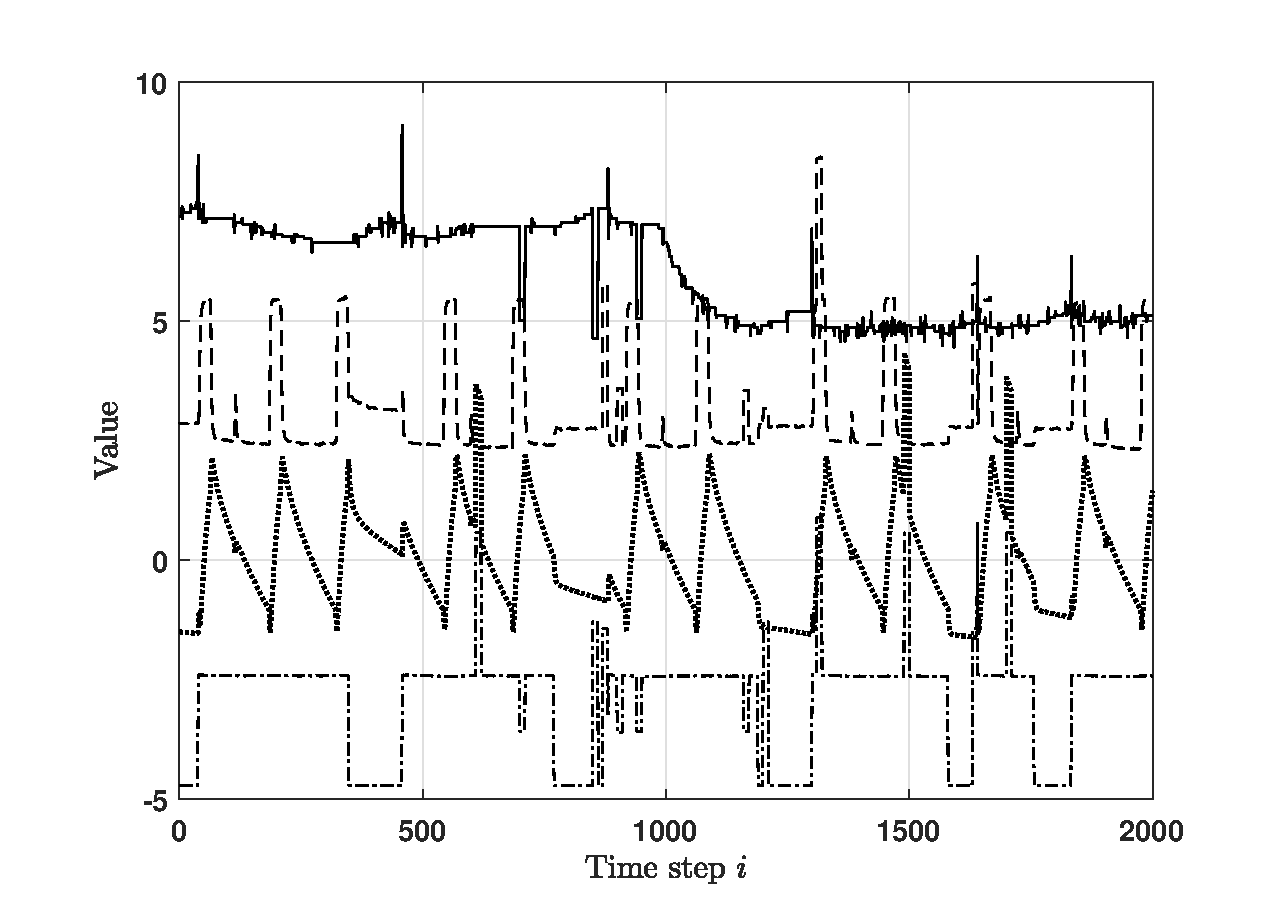
\includegraphics[scale=0.36]{experiments/Experiments_swat_timeseries_outliers}
	\caption{The $4$ time series used from the water treatment plant data set, original (left) and with outliers (right).}
	\vspace{0.2cm}
	\label{fig:experiments_swat}
\end{figure}

Alternatively, a scattermatrix showing all pairwise scatter plots of these $4$ time series can be found in appendix \ref{app:experiments}.

\subsection{Performance metrics and parameters}

For the evaluation on real-world data, we used the same performance metrics as in the previous chapter aside from the number of parameters and preceding data points needed. We left those metrics aside, as we do not focus on criteria of which those metrics are the performance indicators. Besides, the evaluation of the methods with respect to the number of parameters and preceding data points needed are not expected to change much on real-world data. So, we evaluate the method on its detection and runtime performance, with the Area Under the ROC Curve (AUC) and the wall-clock runtime using \texttt{tic} and \texttt{toc} commands in Matlab respectively. 

For $\Delta$RP we kept the parameter $m$ (the number of predictors) low to ensure a low runtime performance. For SPIRIT we slightly explored a range of parameter settings to determine its potential to some extent. However, we kept our exploration of the variance bounds within a sensible range close to the range of $[0.95, 0.98]$ as suggested in \cite{papadimitriou2005streaming}. Table \ref{tab:experiments_parameters} presents the parameter settings used throughout the experiments with real-world data.

\begin{table}[h]
	\centering
	\caption{Parameter settings for the real-world experiments.}
	\label{tab:experiments_parameters}
	\begin{tabular}{l c c}
		\toprule	
		\textbf{Method		}					& \textbf{Parameter			}			& \textbf{Value	}	\\
		\midrule
		\multirow{2}{*}{SPIRIT} 	& $\lambda$						&   $0.97$	\\
										& $[f_{\hat{E}}, F_{\hat{E}}]$	&	$[0.85, 0.95]$ \\
		\midrule
		RP				& $k$							&	$1$			\\	
		$\Delta$RP		& $m$							&	$4$			\\	
		\bottomrule		
	\end{tabular}
\end{table}

\section{Results with water treatment plant data}
\label{sec:experiments_results}

The results of our experiments on the water treatment plant data are presented in table \ref{tab:experiments_results}. The results were averaged over $50$ runs with distinct random projection matrices. Again, results that are significantly better than the opponent(s) according to the \textit{t}-statistic are made bold. 

\begin{table}[h]
	\centering
	\caption{Performances on water treatment plant data.}
	\label{tab:experiments_results}
	\begin{tabular}{l c c }
		\toprule	
		\textbf{Method}		& 	\textbf{AUC }					 	& \textbf{Runtime} 	\\
		\midrule
		SPIRIT		& $0.71$						&  $0.39 (\pm 0.1)$ \\
		RP			& $0.82 (\pm 0.03)$				&  $\mathbf{0.02 (\pm 0.01)}$ \\
		$\Delta$RP	& $\mathbf{0.85 (\pm 0.03)}$	&  $0.31 (\pm 0.06)$ \\
		\bottomrule
	\end{tabular}
\end{table}

For this data, the RP-based methods outperform SPIRIT considering both criteria. The simple RP method with only $1$ projection vector has a significantly better runtime performance as shown in this table. However, it performs little worse in detecting outliers which is caused by its inability of finding contextual outliers. 

As can be seen in figure \ref{fig:experiments_results}, the average ROC curves of the RP method and $\Delta$RP are quite similar. However, if we cannot accept a FPR higher than $0$, the RP method would be a better choice as it yields the highest TPR for FPR $= 0$. If a method is preferred that is able to detect more outliers while minimizing the misclassification costs associated with flagging normal data points as outliers as well, the choice would be the $\Delta$RP method. SPIRIT is probably least desired unless it would be acceptable to incorrectly classify 40\% of the normal data points.

\begin{figure}[h]
	\centering
	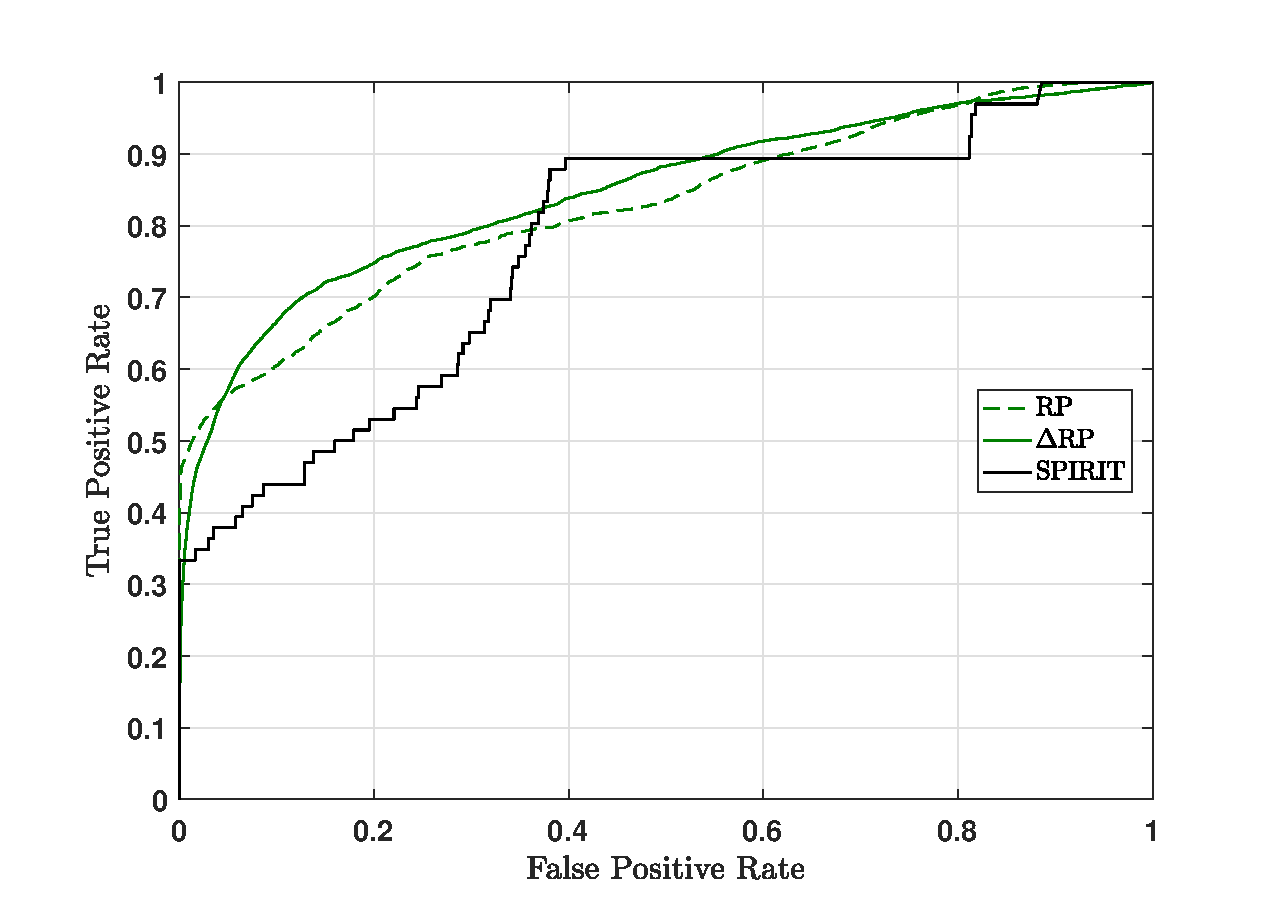
\includegraphics[scale=0.5]{experiments/ROCs_experiments}
	\caption{ROC curves resulting from the experiment with the water treatment plant.}
	\label{fig:experiments_results}
\end{figure}

To shed light on the subtle difference in detection performance of the RP method and $\Delta$RP, we also ran experiments on the same data with only the global or only the contextual outliers. For this experiment, the RP method yields an AUC of $0.99$ for finding the global outliers against $0.98$ for $\Delta$RP and $0.77$ by SPIRIT. However, for the data with only contextual outliers we found an AUC of $0.65$ with the RP method while $\Delta$RP results in an AUC of $0.71$. The AUC obtained by SPIRIT was only $0.36$ explaining its low overall performance of $0.71$. Running PCA offline (when the principal components are learned over the entire data stream) is much better and stable in this case, with an AUC of $0.79$ for global outliers and $0.76$ for contextual outliers. Finally, if we would deploy $\Delta$RP with $m=15$, we can reach an AUC of $0.75$ for the contextual outliers, indicating its unsaturated potential for finding contextual outliers.


\section{Results with non-temporal benchmark data}
\label{sec:experiments_beyond}

As a consequence of the conclusions that the proposed RP-based methods do not exploit temporal relations within time series, and suitable temporal data sets are rarely available online, we also compared our method on non-temporal data sets. Plenty of data sets frequently used for benchmarking unsupervised outlier detection methods are available, which also have more features than our water treatment plant data. As this task does not require an online method we left the online mean and variance estimation aside and deploy $\Delta$RP offline but still unsupervised. This also means that we can compare our method with methods that are not limited to online outlier detection such as the well-known Local Outlier Factor (LOF) which is based on density estimation \cite{breunig2000lof} and offline PCA.

We used $6$ data sets of which the characteristics are described in table \ref{tab:experiments_beyond_data}. These data sets can be retrieved from the UCI Machine Learning repository \cite{uci2018data} as well as the Outlier Detection Dataset repository of Stony Brook University \cite{odds2016}. The data sets used for these experiments all have a clear notion of what is considered normal and abnormal, e.g. data points correspond to healthy persons or persons suffering from a disease (for instance breast cancer or diabetes). 

\begin{table}[h]
	\centering
	\vspace{-0.05cm}
	\caption{Non-temporal benchmark data sets for unsupervised outlier detection.}
	\label{tab:experiments_beyond_data}
	\begin{tabular}{l c c c}
		\toprule	
		\textbf{Method}		& 	\textbf{$\#$ data points $n$}	& \textbf{$\#$ features $d$} & \textbf{$\#$ outliers}	\\
		\midrule
		Mammography	& $11,183$	&   $6$		&	$260 \ (2.3 \%)$	\\
		Thyroid (Ann-)	& $6,832$	&   $6$		&	$534 \ (7.4 \%)$	\\
		Pima		& $768$		&   $8$		& 	$268 \ (35 \%)$	\\
		Breast Cancer Wisconsin (BCW)	& $683$		& 	$9$		&	$239 \ (35 \%)$	\\
		Arrhythmia	& $452$		&	$274$	&	$66 \ (15\%)$		\\
		Ionosphere	& $351$		&	$32$	&	$126 \ (36\%)$	\\
		\bottomrule
	\end{tabular}
	\vspace{-0.05cm}
\end{table}

For the standard RP method we used only one projection vector, i.e. $k=1$, which was observed to yield the best performance. For $\Delta$RP we have set the number of predictors $m$ to $15$ as we are not concerned with optimizing the runtime performance since we compare the performances offline.
The results corresponding to the LOF method were extracted from \cite{liu2008isolation}. They deployed the density-based LOF method with a commonly used parameter $k=10$ reflecting the number of neighbours used in defining the local neighbourhood of each data point. We explored the performance of offline PCA with several variance bounds on all data sets in table \ref{tab:experiments_beyond_data} and set its parameter to a sensible value of $90\%$. For the reconstruction-based methods (RP, $\Delta$RP and PCA) we standardized the data following equation \eqref{eq:experiments_normalization} where we excluded features $j$ of $d$ that have $\sigma_j = 0$.

Table \ref{tab:experiments_beyond} shows the results of this experiment which were averaged over $50$ runs with distinct random projection matrices. Bold scores correspond to the significantly best performance according to the \textit{t}-statistic. The detection performance of the RP method and $\Delta$RP on unstandardized data can be found in appendix \ref{app:experiments}. 

\begin{table}[h]
	\centering
	\vspace{-0.05cm}
	\caption{Detection performances on \textit{standardized} non-temporal data sets.}
	\label{tab:experiments_beyond}
	\begin{tabular}{l c c c c}
		\toprule	
		\multirow{2}{*}{\textbf{Dataset}} & \multicolumn{4}{c}{\textbf{AUC}} \\
		\cmidrule{2-5}
					& \textbf{RP} 						& \textbf{$\Delta$RP} 			&  \textbf{PCA}		& \textbf{LOF}	\\
		\midrule
		Mammography & $\mathbf{0.88 (\pm 0.02)}$		& $\mathbf{0.88 (\pm 0.01)}$	& $0.76$			& $0.67$  	\\
		Thyroid (Ann-)  & $0.67 (\pm 0.00)$ 				& $0.64 (\pm 0.02)$ 			& $0.49$			& $\mathbf{0.72}$	\\
		Pima 		& $\mathbf{0.65 (\pm 0.01)}$ 		& $\mathbf{0.65 (\pm 0.01)}$ 	& $0.57$			& $0.49$	\\	
		BCW  	& $0.95 (\pm 0.01)$					& $\mathbf{0.97 (\pm 0.01)}$ 	& $0.89$			& $0.37$	\\
		Arrhythmia	& $\mathbf{0.77 (\pm 0.00)}$ 		& $0.75 (\pm 0.02)$  			& $0.63$			& $0.73$	\\
		Ionosphere	& $0.79 (\pm 0.00)$ 				& $0.80 (\pm 0.02)$  			& $\mathbf{0.95}$	& $0.89$	\\
		\bottomrule
	\end{tabular}
	\vspace{-0.05cm}
\end{table}

Clearly, the RP-based methods give a quite stable performance considering all data sets, as most AUC's are quite close to the AUC of the best scoring method on a given data set. Only for the Ionosphere data set, the proposed methods perform much worse than PCA and LOF. Overall seen, the RP method and $\Delta$RP are quite comparable in detection performance. Yet the experiments with the unstandardized data point out that the RP method is more sensitive to standardization than $\Delta$RP. 

\section{Conclusions}
In this chapter we exposed the methods to real-world data sets. We examined the methods on (semi-realistic) temporal data for which they were intended. However, we also examined the generalizability of the methods to non-temporal data streams. The reasons for doing so, is that our method actually does not exploit any temporal relations and there is a lack of temporal data sets available that suited our conditions. The main objective of the experiments was to evaluate the methods with regard to the two criteria still open after the analysis. In table \ref{tab:experiments_qualcomp} we provide our conclusions with respect to those two criteria. 
We assigned a `$+$' (plus) in case a method was evaluated as best compared to its opponents given a criterion, or a `$-$' (minus) if its performance was not as good as the best method.

\begin{table}[h]
	\centering
	\vspace{0.1cm}
	\caption{Evaluation based on the experiments.}
	\label{tab:experiments_qualcomp}
	\begin{tabular}{l c c c}
		\toprule
		\textbf{Evaluation criterion} 		& \textbf{RP} 	& \textbf{$\Delta$RP} & \textbf{SPIRIT} \\ \midrule
		Generalizability of performances to different data sets  & $-$ & $+$	& $-$ \\[0.15cm]
		Influence of $d$ and $n$ on	detection performance & $+$ & $+$ & $+$ \\
		\bottomrule		
	\end{tabular}
	\vspace{0.1cm}
\end{table}
 
As observed throughout the analysis and experiments, SPIRIT and the RP method are more sensitive to the mean and range of the data than $\Delta$RP. When it comes to most non-temporal data sets, both RP-based methods outperform a well-known unsupervised outlier detection method based on the Local Outlier Factor and offline PCA. For $4/6$ non-temporal outlier detection benchmark data sets an RP-based method performs better.
In general, $\Delta$RP has shown to yield the most stable performance on synthetic, semi-realistic and real-world data, on temporal and non-temporal, standardized and unstandardized data sets (appendix \ref{app:experiments}).

We could not derive a clear correlation between the detection performance and the dimensionality of the data from the analysis in chapter \ref{chap:analysis} and the experiments in this chapter. Therefore, it seems that the analysed methods are relatively insensitive to the dimensionality of the data. The main problem as identified in section \ref{sec:introduction_complexity}, is that the difference between outlier scores might vanish when $d$ and/or $n$ become large \cite{beyer1999nearest}. But Zimek et al. \cite{zimek2012survey} already found that the dimensionality might not significantly affect outlier detection methods that compute outlier scores based on the Euclidean distance. This statement might hold for methods that compute outlier scores from the squared Euclidean distance as well. Therefore we also ran some small experiments with taking the squared Euclidean norm of each data point directly as outlier score. This measure appeared to be very effective for global outliers, but does not work for contextual outliers. Yet if one wants to find global outliers in extremely high-dimensional data sets, the squared Euclidean distance seems already relatively insensitive to the curse of dimensionality.


